\batchmode
\documentclass[a4paper,10pt]{article}
\usepackage{graphicx}
\usepackage{fancyvrb}
\usepackage{color}
\usepackage{xcolor}
\usepackage{verbatim}
\usepackage{amssymb}
\usepackage{amsmath}
\usepackage{hyperref}
\usepackage{natbib}
\usepackage{caption}
\usepackage{subcaption}
%\usepackage{subfigure}
\hypersetup{urlcolor=blue, colorlinks=true} 
\usepackage{float}

%used in SL section
\usepackage{mathptmx}
%\usepackage{siunitx} %SI-einheiten
\usepackage{lmodern} %weitere mathematischen Symbole
\usepackage{placeins} %floatbarrier

%\DeclareSIUnit\parsec{pc}
%\DeclareSIUnit\lightyear{ly}
%\DeclareSIUnit\year{yr}
%\DeclareSIUnit\erg{erg}
%\DeclareSIUnit\ster{ster}
%\DeclareSIUnit\arcsec{arcsec}
%\DeclareSIUnit\deg{deg}


\definecolor{gruen}{cmyk}{0.35,0.01,0.80,0.1}

\textheight=25.5cm
\textwidth=17.5cm
\voffset=0.cm
\hoffset=-0.0cm
\oddsidemargin -1cm
\evensidemargin -1cm
\topmargin -2cm
\baselineskip=0.900cm
\setlength{\parindent}{0in}
\setlength{\parindent}{1cm}

\graphicspath{{Figures/}}

\providecommand{\e}[1]{\ensuremath{\times 10^{#1}}}
\newcommand{\given}[2]{\ensuremath{P(#1|#2)}}
\newcommand{\x}[0]{\ensuremath{\vec{x}}}
\newcommand{\gauss}[3]{\ensuremath{\frac{1}{\sqrt{2\pi#2^2}}\text{exp}\left(- \frac{(#1-#3)^2}{2#2^2}\right)}}
\newcommand{\cosmos}{COSMOS}
\newcommand{\xmmlss}{XMM-LSS}
\newcommand{\cdfs}{CDFS}
\newcommand{\elais}{ELAIS-S1}
\newcommand{\spt}{SPT DEEP}
\newcommand{\ddfa}{DDF\_820}
\newcommand{\ddfb}{DDF\_858}
\newcommand{\ddfc}{DDF\_1200}
\newcommand{\ddfd}{DDF\_2689}
\newcommand{\feature}{feature\_baseline\_10yrs}
\newcommand{\strech}{$X_1$}
\newcommand{\sncolor}{$c$}
\newcommand{\daymax}{$T_0$}
\newcommand{\redshift}{$z$}
\newcommand{\tmin}{$T_{min}$}
\newcommand{\tmax}{$T_{max}$}
\newcommand{\phasemin}{$ph_{min}$}
\newcommand{\phasemax}{$ph_{max}$}
\newcommand{\tgapcosmos}{$T_{gap}^{\cosmos}$}
\newcommand{\tgapothers}{$T_{gap}^{others}$}
\newcommand{\zlimit}{$z_{\mathrm{limit}}$}
\newcommand{\zfaint}{$z_{\mathrm{faint}}\ $}
\newcommand{\nsnfaint}{$N_{z<z_{\mathrm{faint}}}\ $}
\newcommand{\zmed}{$z_{\mathrm{med}}\ $}
\newcommand{\nsnmed}{$N_{z<z_{\mathrm{med}}}\ $}
\newcommand{\FixMe}[1]{{\color{red} \bf \large #1}}
\newcommand{\opsim}{{\tt OpSim\ }}
\newcommand{\slair}{{\tt SLAIR\ }}
\newcommand{\altschedsched}{{\tt AltSched\ }}
\newcommand{\altsched}{{\tt altsched\ }}
\newcommand{\myparagraph}[1]{\paragraph{#1}\mbox{}\\}
\newcommand{\sne}{{SNe Ia}}


\def\mybox(#1,#2){\begin{center}
\fbox{
{\bf
\begin{minipage}{0.8\textwidth}
     \begin{center}
\vspace*{0.2cm}
           #1\\
\vspace*{0.2cm}
          #2
     \end{center}
\end{minipage}
}}

\end{center}
\vspace{0.2cm}
}


% used in SL section
\newcommand{\todo}[2]{\textcolor{red}{\textbf{TODO (#1): #2}}}

\title{Summary of final assessment for the white paper call}
\author{DESC Supernovae Working Group \\ 
\\
T. Allam Jr.,R.Biswas, J.Carrick, Ph.Gris, R.Hlo\v{z}ek, I.Hook, A.Kim, M.Lochner \\ J.McEwen, H. Peiris, N.Regnault, R. Schuhmann, D.Scolnic, C.N.Setzer}
\date{}


\begin{document}
\maketitle

\newpage
\vspace*{10cm}
\newpage

\noindent
The working group has developed the following set of metrics to evaluate the proposed observing strategies:
\begin{itemize}
\item Number of well-measured Type Ia supernovae (WFD and DDF)
\item w0-wa Figure of Merit (WFD and DDF)
\item Photometric classification (DDF)
\item Peculiar velocity (WFD)
\item Overlap wit 4MOST extragalactic surveys (WFD)
\end{itemize}

\noindent
From these metrics a ranking of observing strategies has been done (Table \ref{tab:summary}).


\begin{table}[!htbp]
  \begin{center}
    \caption{Ranking of observing strategies (top 5 and worst 5) according to metric scores.}\label{tab:summary}
\begin{tabular}{c|l|l}
  \hline
  \hline
Metric  & \multicolumn{1}{c|}{Top 5} & \multicolumn{1}{c}{Worst 5} \\
\hline
\hline
%%%%% NSN
{\bf $N_{SN}$ (well-sampled)}  &                                          & \\
                               & 1. altsched/altsched wide                & 1. feature\_baseline\_10yrs\\
WFD                            & 3. Rolling mix                           & 2. blobs same zmask\\
                               & 4. colossus\_2667                        &  3. blob same\\
                               & 5. feature\_rolling\_2/3                 & 4. pontus\_2002 \\
                               &                                          &  5. minion\_1016 \\
\hline
                               & 1. kraken\_2035/feature\_baseline\_10yrs &  1. kraken\_2036\\
DDF                            & 3. colossus\_2665                        &  2. mothra\_2045 \\
                               & 4. colossus\_2667                        &  3. pontus\_2489\\
                               & 5. pontus\_2002                          &  4. colossus\_2664\\
                               &                                          &  5. baseline\_2018a  \\
\hline
%%%%% w0wa
{\bf w0wa FoM}                 & 1. kraken\_2035                          &  1. nexus\_2097\\
                               & 2. colossus\_2667                        &  2. mothra\_2049\\
WFD+DDF                        & 3. pontus\_2489                          &  3. pontus\_2002\\
                               & 4. colossus\_2026                        &  4. kraken\_2044 \\
                               & 5. kraken\_2042                          &  5. colossus\_2664\\
\hline
%%%%% photometric classification
{\bf Photometric}              & 1. pontus\_2489/kraken\_2042             &  1. kraken\_2044 \\
{\bf Classification}           & 3. colossus\_2665                        &  2. kraken\_2036\\
      DDF                      & 4. mothra\_2045                          &  3. kraken\_2035\\
                               & 5. colossus\_2667                        &  4. kraken\_2026\\
      \hline

%%% peculiar velocity 
{\bf Peculiar velocity I}      & 1. altsched                              &  1. feature\_baseline\_10yrs \\
                               & 2. altsched\_twilight                     &  2. blobs same zmask\\
      WFD                      & 3. kraken\_2044                           &  3. blob same\_10yrs \\
                               & 4. colossus\_2667                        &  4. minion\_1016\\
                               & 5. pontus\_2489                          &  5. feature\_rolling\_1/2\\
      \hline
%%% peculiar velocity 
{\bf Peculiar velocity II}     & 1. kraken\_2044                          &  1. nexus\_2097\\
                               & 2. colossus\_2667                        &  2. mothra\_2049 \\
      WFD                      & 3. pontus\_2489                          &  3. colossus\_2665 \\
                               & 4. pontus\_2002                          &  4. kraken\_2026 \\
                               & 5. kraken\_2042                           &  5. colossus\_2664 \\
      \hline
%%%%% Overlap 4MOST

 {\bf Overlap with 4MOST}      & 1. pontus\_2002                          &  1. colossus\_2667, kraken\_2026, pontus\_2489\\
                               & 2. colossus\_2665                        &  \\
   WFD                         & 3. colossus\_2664                        &   \\
     \hline
\end{tabular}
\end{center}
\end{table}

\noindent Lessons learned from this exercise may be summarized as follow:

\paragraph{Primary metric} 

Among the set of metrics considered in this study one of the most sensitive to the features of observing strategies (ie the key facets cadence, season length, depth, spatial coverage and uniformity) is probably the number of well-measured \sne~in combination with the redshift limit of the survey \zlimit. In fact all other metrics (except the one related to synergy with 4MOST) rely on a high-quality \sne~sample. The w0-wa Figure of Merit is usually used to assess the quality of observing strategies because it can easily be compared and/or combined with other Dark Energy probes. But this metric is not as sensitive as the number of well-measured \sne. We thus think that the primary metric to assess the quality of observing strategies should be the number of well-measured supernovae combined with the redshift corresponding to the completeness of the survey.


\paragraph{Conclusion about proposed observing strategies}

Table \ref{tab:summary} is a ranking of the best and worst observing strategies according to metric scores. One may notice that some of the metrics did not consider all the possible available cadences: $w0-wa$ FoMs and Peculiar velocity (II) were not evaluated with \altsched simulations and the photometric classification did not consider \feature\footnote{Some of these cadences are beeing processed.}. Nonetheless the conclusion that may be drawn from Table \ref{tab:summary} is that the best cadences for SN science among the proposal are:
\begin{itemize}
\item WFD: \altsched-like simulations corresponding to surveys with high cadences in the $griz$ bands (at the level of few days), with low inter-night gap variations, over a large area (at least 18000 $deg^2$) 

\item DDF: \feature-like simulations corresponding to Deep Drilling Fields observed with a regular cadence of 3 days with low inter-night gap variations, and with long seasons (typically 160 to 180 days). 
\end{itemize}

Two key points are thus very important for SN science: a high and regular cadence. This is what drives the results in the WFD survey. The season length is also important in the DD mini-survey to collect a larger sample of well-measured \sne. 

\paragraph{Observing strategy and scheduler}

The results presented below tend to show that the main features related to simulated strategies (the key points mentioned above) may be quite different from one simulation to another. In particular \altsched scheduler tend to propose WFD surveys that lead to very good performance in terms of number of well-measured \sne~and \zlimit. We have made further studies to understand the reason of this result by comparing some of the outputs of \opsim and \altsched(Table \ref{tab:opsim_vs_altsched}). It is very likely that the differences found between the two schedulers have as origin the methods used to observed the sky: \opsim relies on a greedy algorithm that minimizes slew times and optimizes observing conditions; \altsched performs a systematic scan at the meridian of a predefined (Ra,Dec) area with a larger number of filter changes every night. The method used by \altsched seems to lead to very interesting cadences for SN science. Additional studies are nonetheless necessary to evaluate the impact of e.g. uncovered areas or observations when the Moon is up on \altsched performance.

\begin{table}[!htbp]
  \begin{center}
    \caption{Comparison of \opsim and \altsched outputs}\label{tab:opsim_vs_altsched}
\begin{tabular}{c|c|c}
  \hline
  \hline
 & \altsched & \opsim \\
 \hline
 Season length [days] & $\sim$ 150 & 130 to 180 \\
 \hline
 Effective cadence [days]   &        & \\
 				           g &  14  & 23 \\
 				           r &   6  & 14 \\
						   i &   8  & 14 \\
						   z &   7  & 15 \\
 \hline
 Filter allocation 			&  & \\
 				            u & 8\% & 6-8\% \\
 					  		g &  11\% & 9-10\% \\
 				           r &   28\%  & 20-22\% \\
						   i &   18\%  & 21-22\%\\
						   z &   26\%  & 18-21\% \\
						   y &   9\%  & 19-25\% \\
 \hline
 \# filter changes per night      & & \\
 				          median & 12 & 2 \\ 
 				          min    & 2 & 0-2\\
 				          max    & 18 & 11-20 \\
 \hline
 Observations @low Moon distance & yes (except for u-band)& no \\
                                 & 10 to 15\% of the visits & \\
 \hline
 Observations @meridian          & yes    & yes \\
 \hline
 				               & North Ecliptic Spur & \\
 Uncovered areas 			& North Galactic Plane & \\
 							     & South Celestial Pole &  \\
 \hline
 \end{tabular}
\end{center}
\end{table}

\paragraph{Parameters for close-to-optimal cadences} The metrics considered in this study allowed us to rank the proposed observing strategies and thus to outline what the parameters of a close-to-optimal cadence would be for SN science. The list of the key points is given in Table \ref{tab:optimal_strategy}

\begin{table}[!htbp]
  \begin{center}
    \caption{Key facets of a close-to-optimal observing strategy for SN science.}\label{tab:optimal_strategy}
\begin{tabular}{c|c|c}
  \hline
  \hline
 Key facet & WFD & DDF \\
 \hline
a) Cadence                      & 10(g),5(r),6(i),6(z) days & 1 to 2 days (filter sequence splitting) \\
b) Season length                & $\sim$ 150 days               & 180 to 200 days \\
c) Filter allocation            & mostly g,r,i,z            & mostly g,r,i,z (y to be quantified) \\
d) Coverage                     & $\geq$ 18000 $deg^2$ provided a), b) and c) & 5 DDF - 1 ultra-deep \\
e) Rolling cadence              & if necessary for a), b) and c) to happen & \\
f) Revisit same band same night & no & \\
g) Uniformity                   & yes & \\
\hline
 \end{tabular}
\end{center}
\end{table}




\newpage

%% Number of well-measured SN - WFD
\mybox(Number of well-measured supernovae/Survey completeness,WFD)

We propose to use as a primary metric the size and depth of a the subset of well-sampled \sne using the redshift limit \zfaint (\zmed) as the limit beyond which the faintest\footnote{A faint \sne~is defined by (\strech = -2.0,\sncolor = 2.0) and a medium one by (\strech=0.0,\sncolor=0.0) where \strech~and \sncolor~are the stretch and color, respectively} (medium) \sne~no longer passes light curve requirements\footnote{Main light curve requirements: good quality measurements in at least three bands;  phases in [-10;+30]; 5 (10) visits before (after) peak; $\sigma_C<$ 0.04 where $\sigma_C$ is the error on the color; all observations satisfying 380 nm $~<~\bar{\lambda}_{obs}/(1+z)~<$ 700 nm.} and \nsnfaint (\nsnmed), the number of well-sampled supernovae below this redshift. The former give an assessment of the size and depth of the redshift limited sample, i.e. the sample of supernovae usable for cosmology, and whose selection function is extremely easy to determine.  The latter gives an assessment of the size and depth of the sample of SNe
that will have precise distances.

WFD observations involve a large number of fields.  The observations
are dithered, and the size and depth of the final sample depends
heavily on the details of the observing strategy (in particular, the
filter allocation strategy and the field selection function \ldots). Instead of performing full (time-consuming) simulations, we opted for a slightly different approach, which we describe below.

The celestial sphere is pixellized in Healpix superpixels\footnote{we
  choose nside=64, which corresponds to 0.8 deg$^2$ healpixels.  We
  have verified that (1) larger pixels (nside=32) leads to
  underestimating the number of SNe by $\sim$ 15\% and
  that smaller pixels (nside=128 and above) give exactly the same
  results.}.  The directions / healpixel affected by a Galactic extinction $E(B-V)$ larger than 0.25
are masked and not included in our assessment. We consider only the $griz$ observations which are the ones
that matter to derive SN luminosity distances. 
Using a simple model of the LSST focal plane, we play
the cadence, and determine, the list of superpixels observed for a
given exposure. This allows us to build a log which reports the mjd,
band, and observing conditions of each healpixel observation.

We can then analyze this log, using as a probe, a fiducial SN~Ia,
e.g. the faint or medium \sne. For each mjd and each pixel, we determine:
\begin{eqnarray}
  z_{\mathrm{lim}} & = & \mathrm{max}\left(z | \mathrm{LC(z)\ fulfill\ requirements}\right) \\
  N_{z<z_{\mathrm{lim}}} &= & \delta\Omega_{\mathrm{pix}} \int_0^{z_\mathrm{lim}} \frac{\Delta T_{\mathrm{step}}}{1+z}\ {\mathcal{R}}(z)\ dV(z)
\end{eqnarray}
where $\delta\Omega_{\mathrm{pix}}$ is the solid angle subtended by
one pixel, $\Delta T_{\mathrm{step}}$ is the simulation time step (in
observer frame days) and $\mathcal{R}(z)$ is the SN~Ia volumetric rate \cite{perrett}.  We also
compute the average cadence (in day$^{-1}$), i.e. the number of $g, r,
i$ or $z$ visits in a fiducial restframe interval.


The quantities above are determined for each pixel and each night
(identified by its mjd) and may be reported in full sky maps, which give
an assessment of how the cadence performs in a $\sim 50$ day time
interval around the current mjd. From these maps, we can build global
maps giving, as a function of the position on the sky (1) the density
of supernovae (2) the median maximum redshift (3) the median cadence.
The results reflect the proposed observing strategy features (such as the median cadence, inter-night gaps, depth, season length, space coverage). For some of the cadences, especially the rolling ones, the average properties (size and
depth) of the SN sample vary significantly as a function of the sky
direction. Some of these effects are related to seasonality (better
seeing allows to go deeper, for example) and depend on how realistic
the \opsim weather and seeing logs are. Others are clearly artefacts
of the observing cadence and can be corrected. For example, {\tt Mothra} and {\tt SLAIR} rolling cadences show lines clearly
visible which correspond to depleted regions at the boundary between
the areas observed each year. The same is true on altsched rolling,
which also displays a strongly depleted region, at the region where
the scheduler switches between the upper and lower declination area.

Our primary metrics, ($z_{\mathrm{faint|median}}$, $N_{\mathrm{faint|median}}$) can be derived from these
maps.  Figure \ref{fig:nsn_zmax_med}
gives a synthetic presentation of our cadence evaluation, in the planes
(\zfaint, \nsnfaint) and (\zmed, \nsnmed), respectively. The rolling version of \altsched is the best performing cadence.  It will allow us to build a
very deep sample \zmed $\sim 0.45$ of more than well sampled 300,000
SNe.  {\tt altsched} covers more area, at the expense of a lower
cadence.  As a consequence, it is not as deep, but allows to obtain a
larger number of well-sampled SNe.

\begin{figure}[htbp]
  \begin{center}
    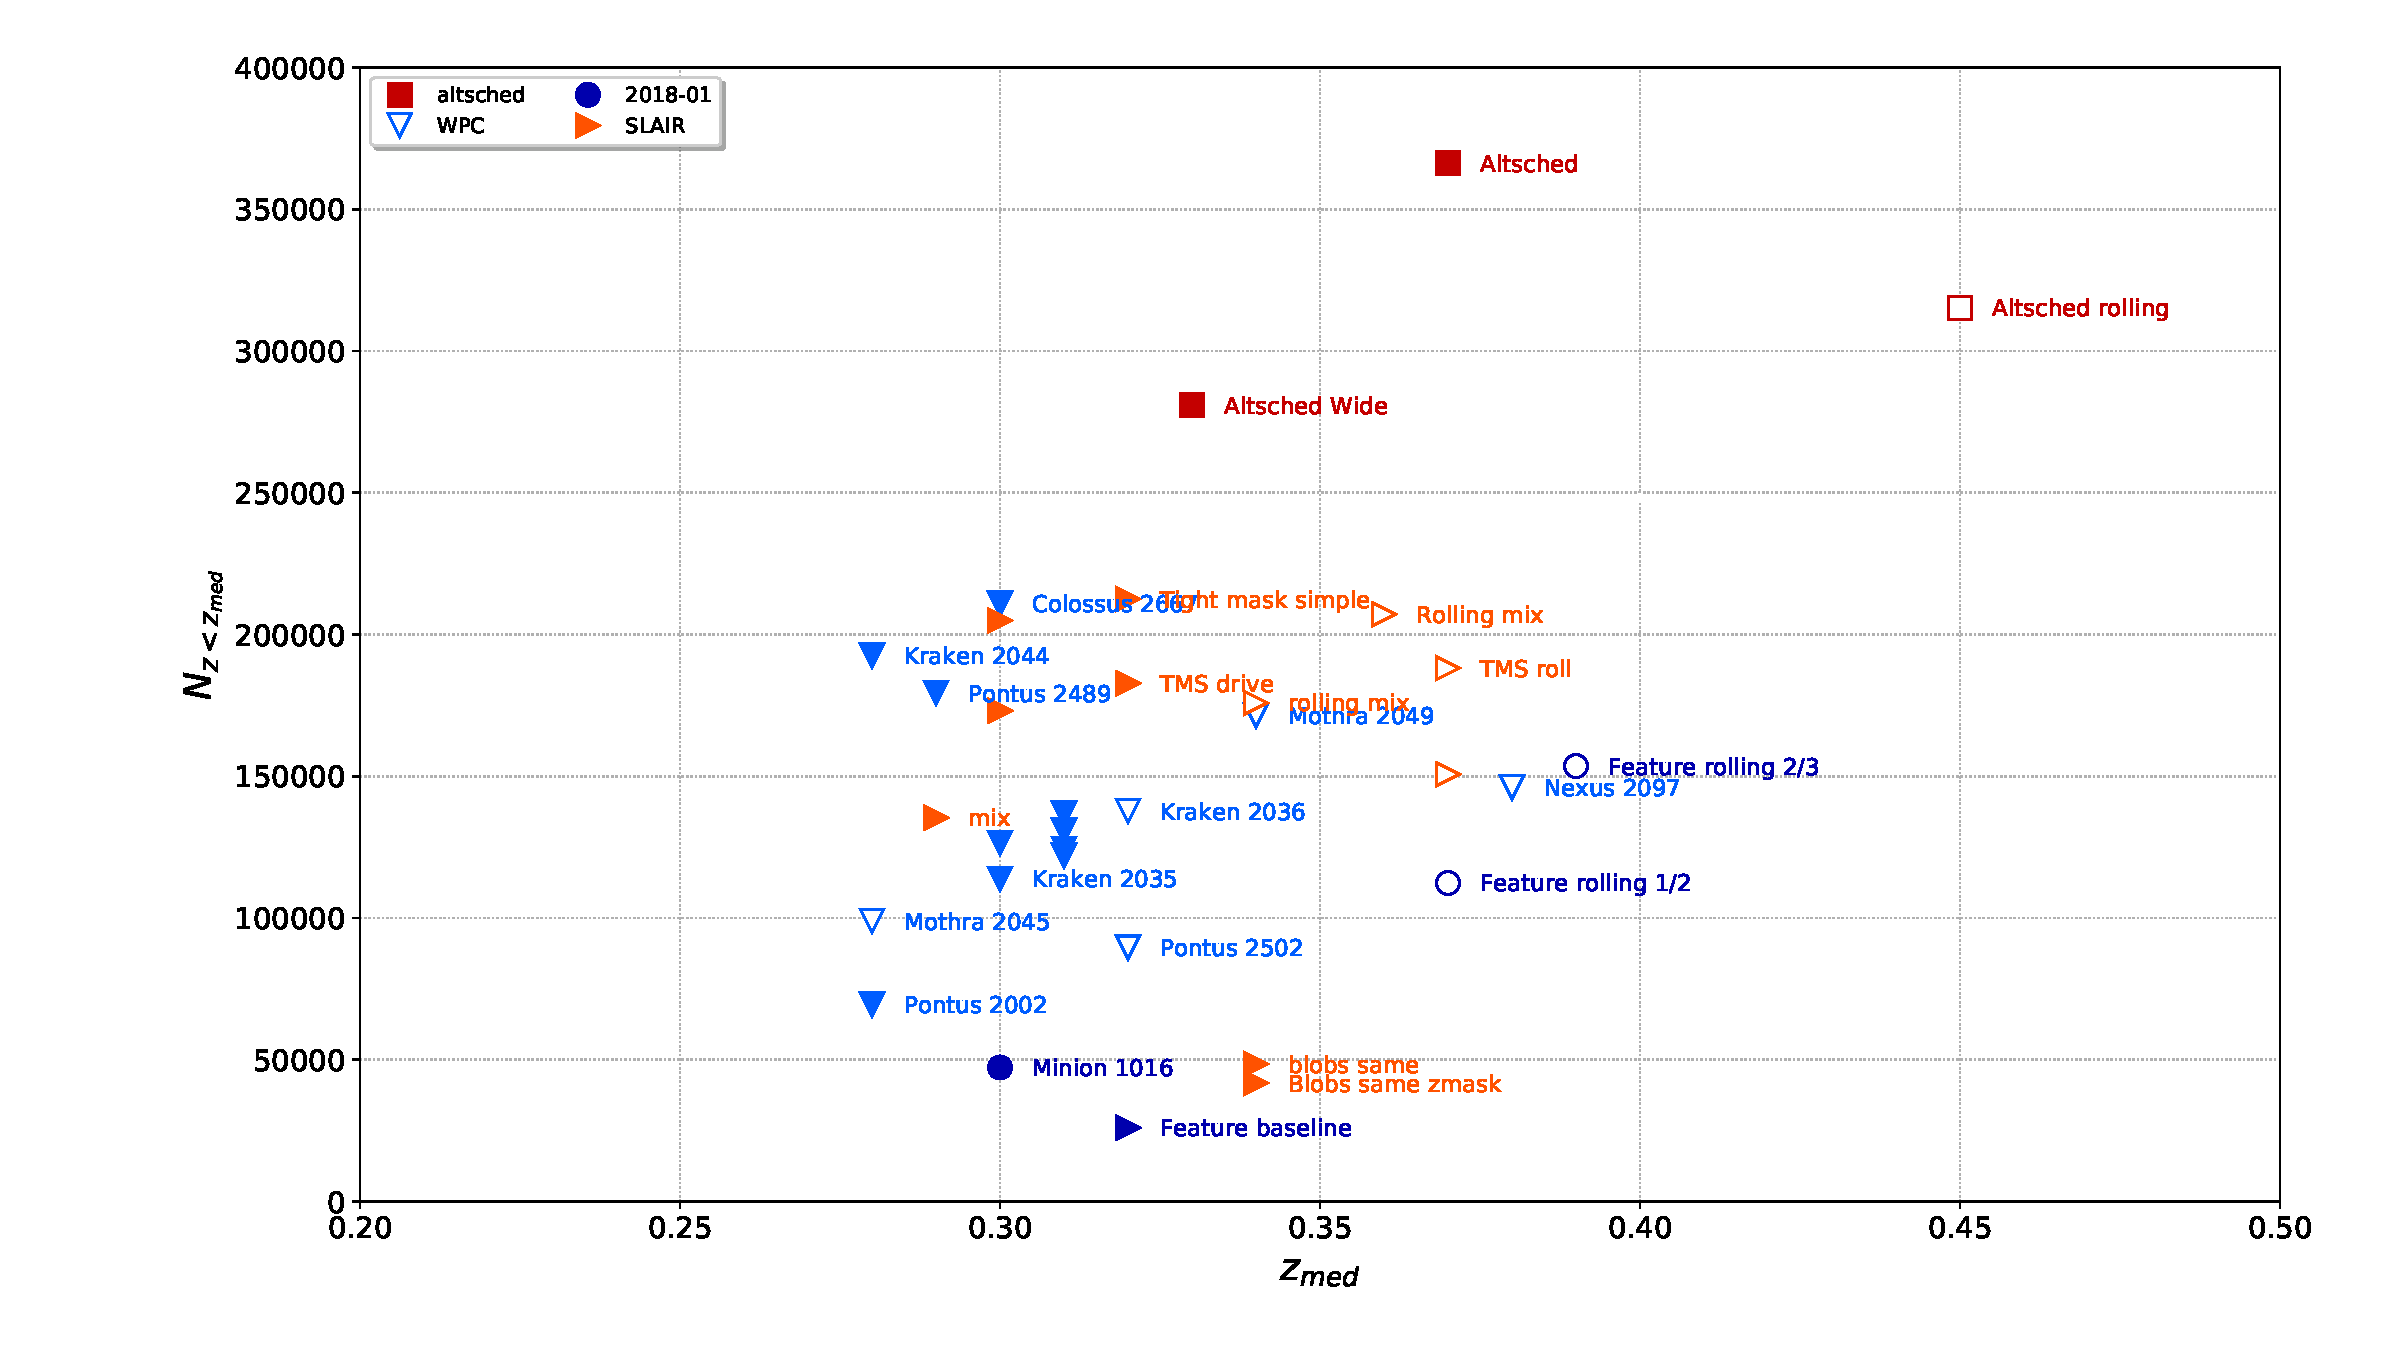
\includegraphics[width=\linewidth]{summary_plot_wfd_mediansn.pdf}
    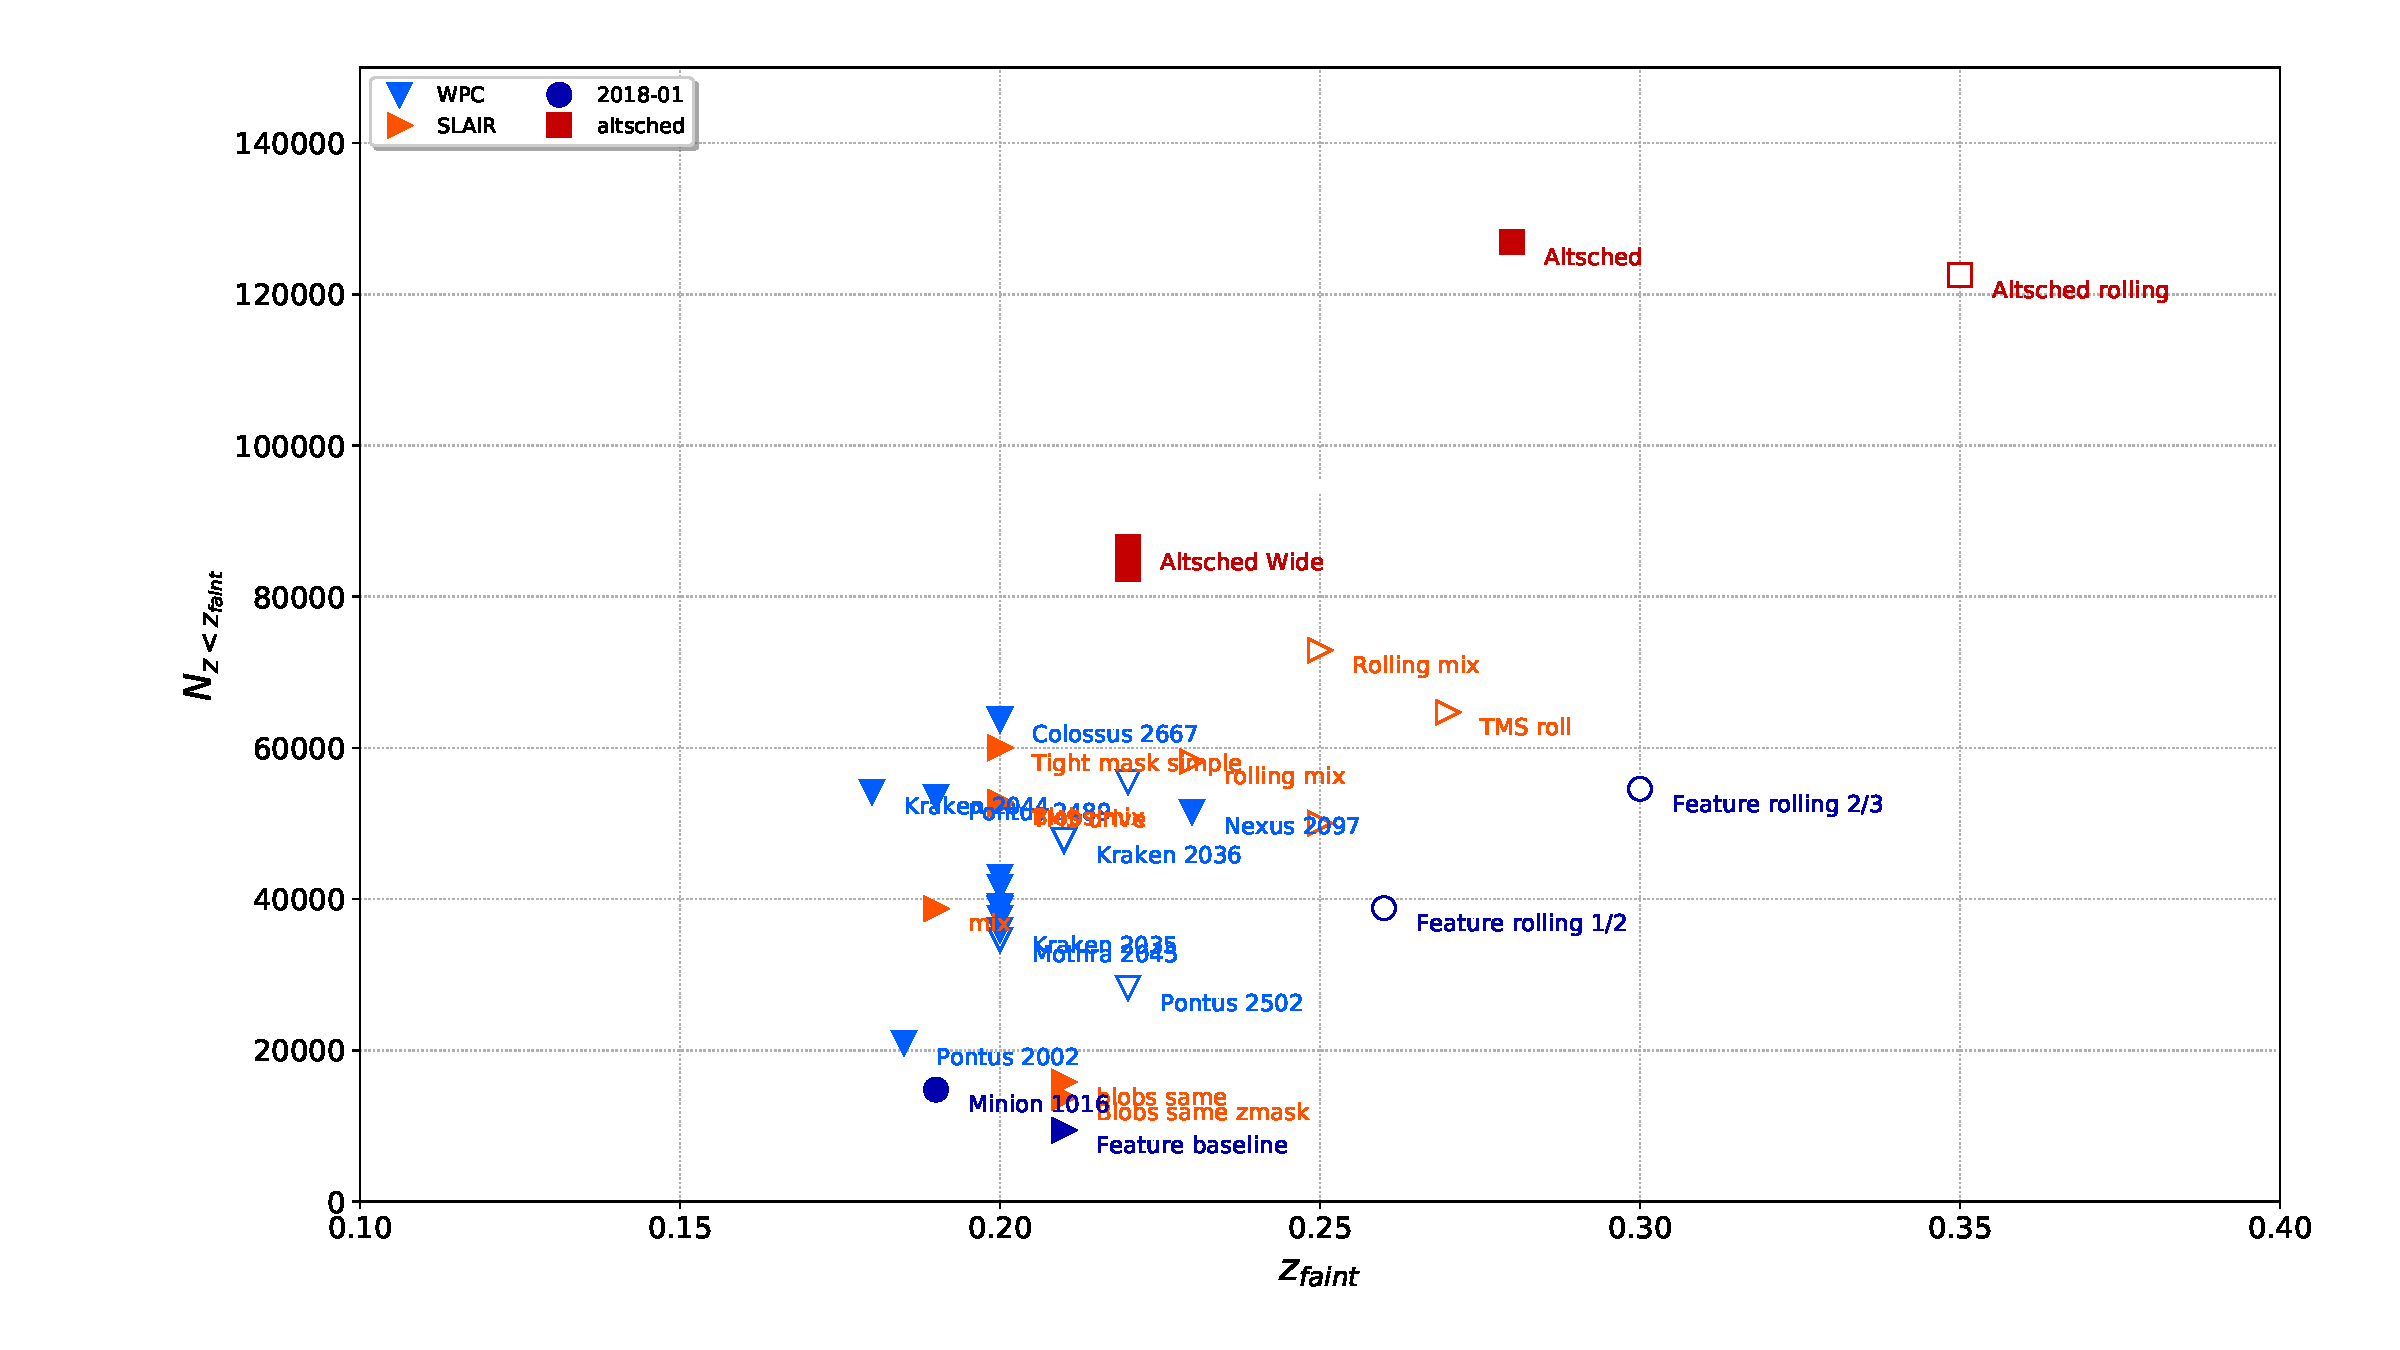
\includegraphics[width=\linewidth]{summary_plot_wfd_faintsn.pdf}
    \caption{Representation of the cadences analyzed in this study in
      the plane (\zmed, \nsnmed) (top) and (\zfaint, \nsnfaint) (bottom).}
    \label{fig:nsn_zmax_med}
  \end{center}
\end{figure}

Most of the cadences released for the white paper call do not allow to
go as deep, no to secure as many well sampled SNe. The best \opsim and
\slair rolling cadences allow to reach redshift limits that are
similar to the non-rolling version of \altsched and yield samples that
are about 40\% smaller. Why simulations with the feature-based scheduler ( {\tt rolling mix} and {\tt tms roll}) do not reach the
performance of {\tt altsched rolling} is unclear at this point and is
being investigated.



\newpage

%% Number of well-measured SN - DDF
\mybox(Number of well-measured supernovae/Survey completeness,DDF)

The DDF  observations involve a  small number of fields  and $O(10^4)$
SNe. The list of simulated DDF is given in table
\ref{tab:ddf_list}. The location of four DDF (\cosmos, \xmmlss, \cdfs~and \elais) has already been chosen by the project. The number of considered DDF ranges from 4 to 9.


\begin{table*}[!htbp]
  \caption{List and location of Deep Drilling Fields observed. \cosmos, \xmmlss, \cdfs~and \elais~ have been considered by all (but \altschedsched-like) simulations. \spt~ was not simulated in \feature. \ddfa, \ddfb, \ddfc, \ddfd~were simulated in kraken\_2035 only.}\label{tab:ddf_list}
  \begin{center}
  \begin{tabular}{lcc||lcc}
    \hline
    \hline
    Field name & Ra (deg) & Dec(deg) & Field name & Ra (deg) & Dec(deg) \\
    \hline
    \hline
    \cosmos & 150.36 & 2.84 & \ddfa  & 119.55 & -43.37 \\
    \xmmlss & 34.39 & -5.09   & \ddfb  & 187.62 & -42.49 \\
    \cdfs & 53.00 & -27.44  & \ddfc  & 176.63 & -33.15\\
    \elais & 0.  & -45.52  & \ddfd 9 & 201.85 & 0.93\\
    \spt  & 349.39 & -63.32 &&&\\
  
    \hline
  \end{tabular}
 
  \end{center}
\end{table*}

DDF observations are composed of sequences of 96 visits\footnote{u band visits are also available but were not considered.}  (in a row) in r,g,i,z,y bands (namely 20, 10, 20, 26, 20 visits). This corresponds to a total observing time of about one hour and few minutes if filter changes, slew times and telescope overheads are taken into account.

The strategy to estimate the number of well-measured type Ia supernovae may be summarized in four steps: (1) light curves are simulated\footnote{Simulator: SNCosmo ; simulation parameters: \strech~$\in$ [-2.0, 0.0, 2.0], \sncolor~$\in$ [-0.2, 0.0, 0.2], Daymax $\in$ [$T_{obs}^{min},T_{obs}^{max}$] - step: 0.1 day, $z$ $\in$ [0.01,1.4]- step 0.025} and fitted using observations of a given cadence; (2) selection criteria are applied to get high-quality supernovae; (3) the resulting observing efficiency curves are then convolved with a production rate \cite{perrett} so as to estimate the number of well-measured type Ia supernovae that may be collected by LSST given an observing strategy. 

 The selection of a sample of well-measured type Ia supernovae is done in two steps. A sample of observable supernovae is selected by requiring light curves to have \phasemin $\leq$ -5 and \phasemax $\geq$ 20 (where \phasemin~ and \phasemax~ are the minimal and maximum phases of the LC points, respectively). For each supernovae in this reference sample, additional selection criteria are applied (the number of points before and after the maximum is higher than 4 and 10, and $\sigma_c$, the error on the \sncolor~parameter estimated from the fit of the light curve, is lower than 0.04). The season length which depends on the redshift is estimated using the supernovae of the reference sample.


\begin{figure}[htbp]
  \begin{center}
    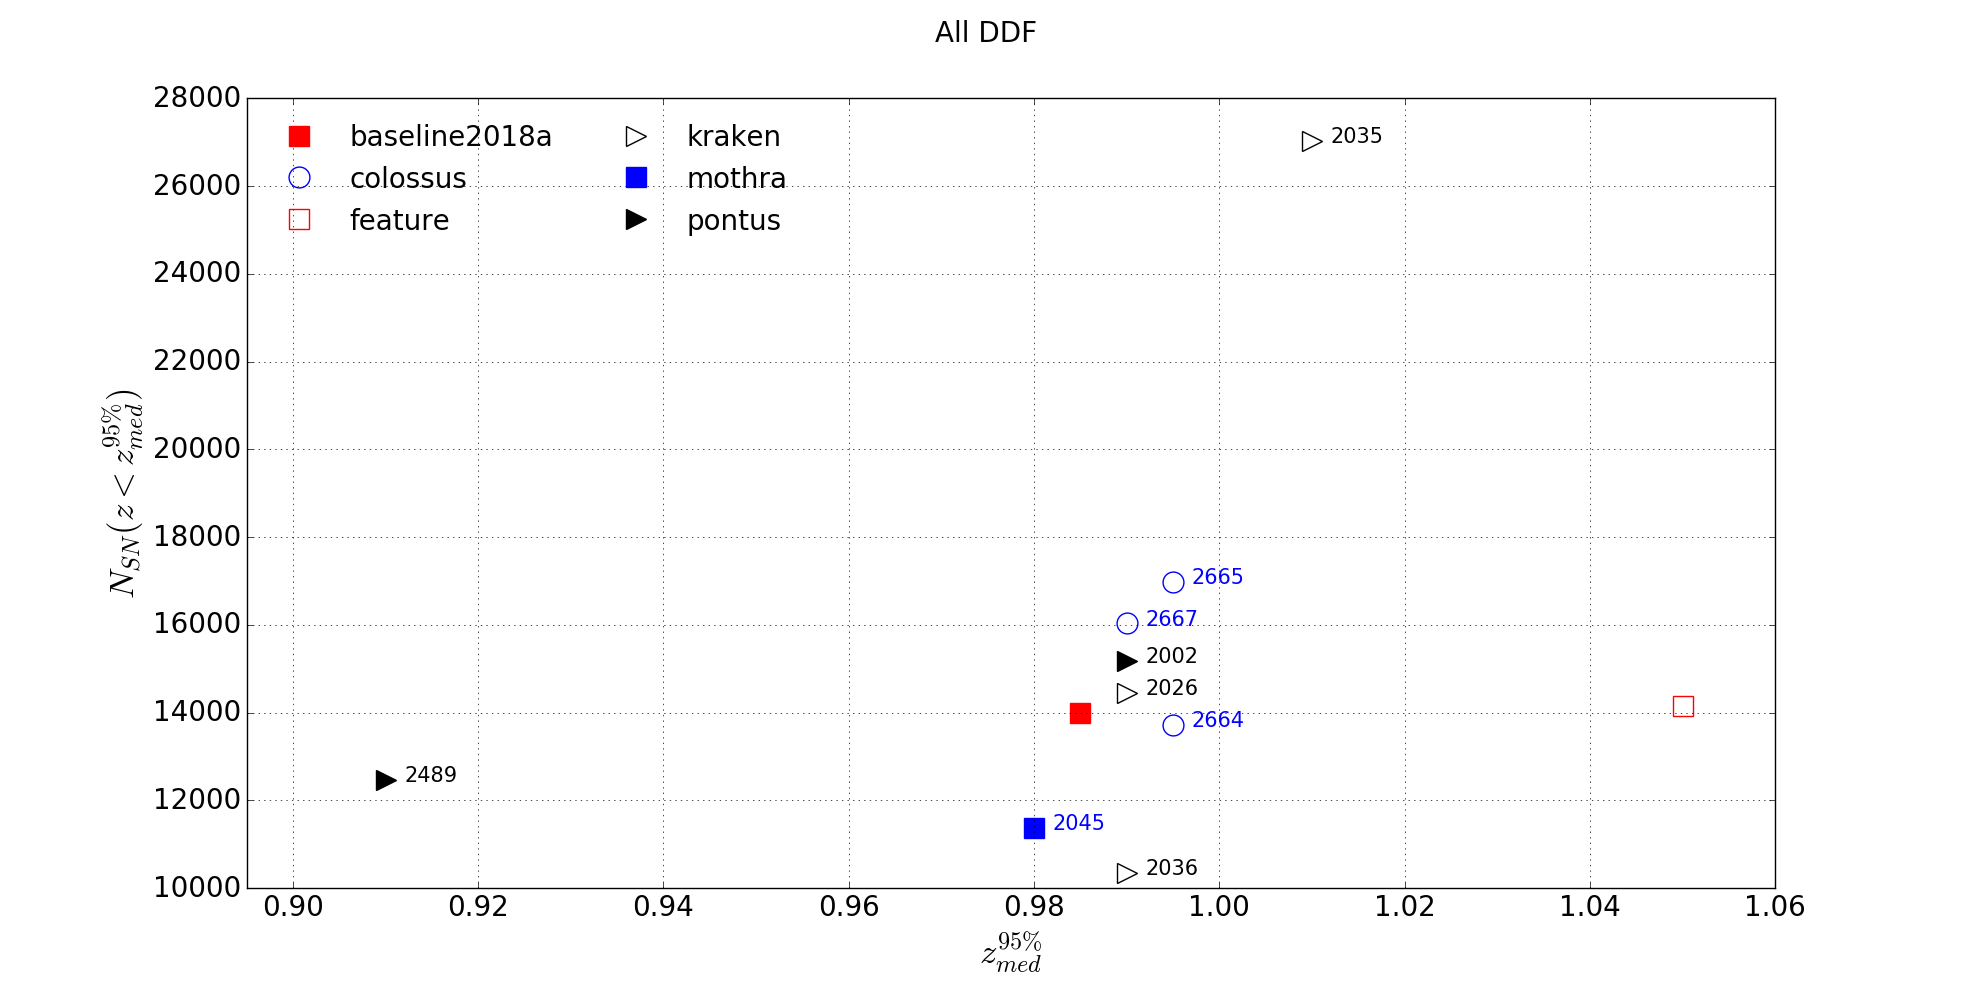
\includegraphics[width=\linewidth]{Z95_NSN_med.png}
    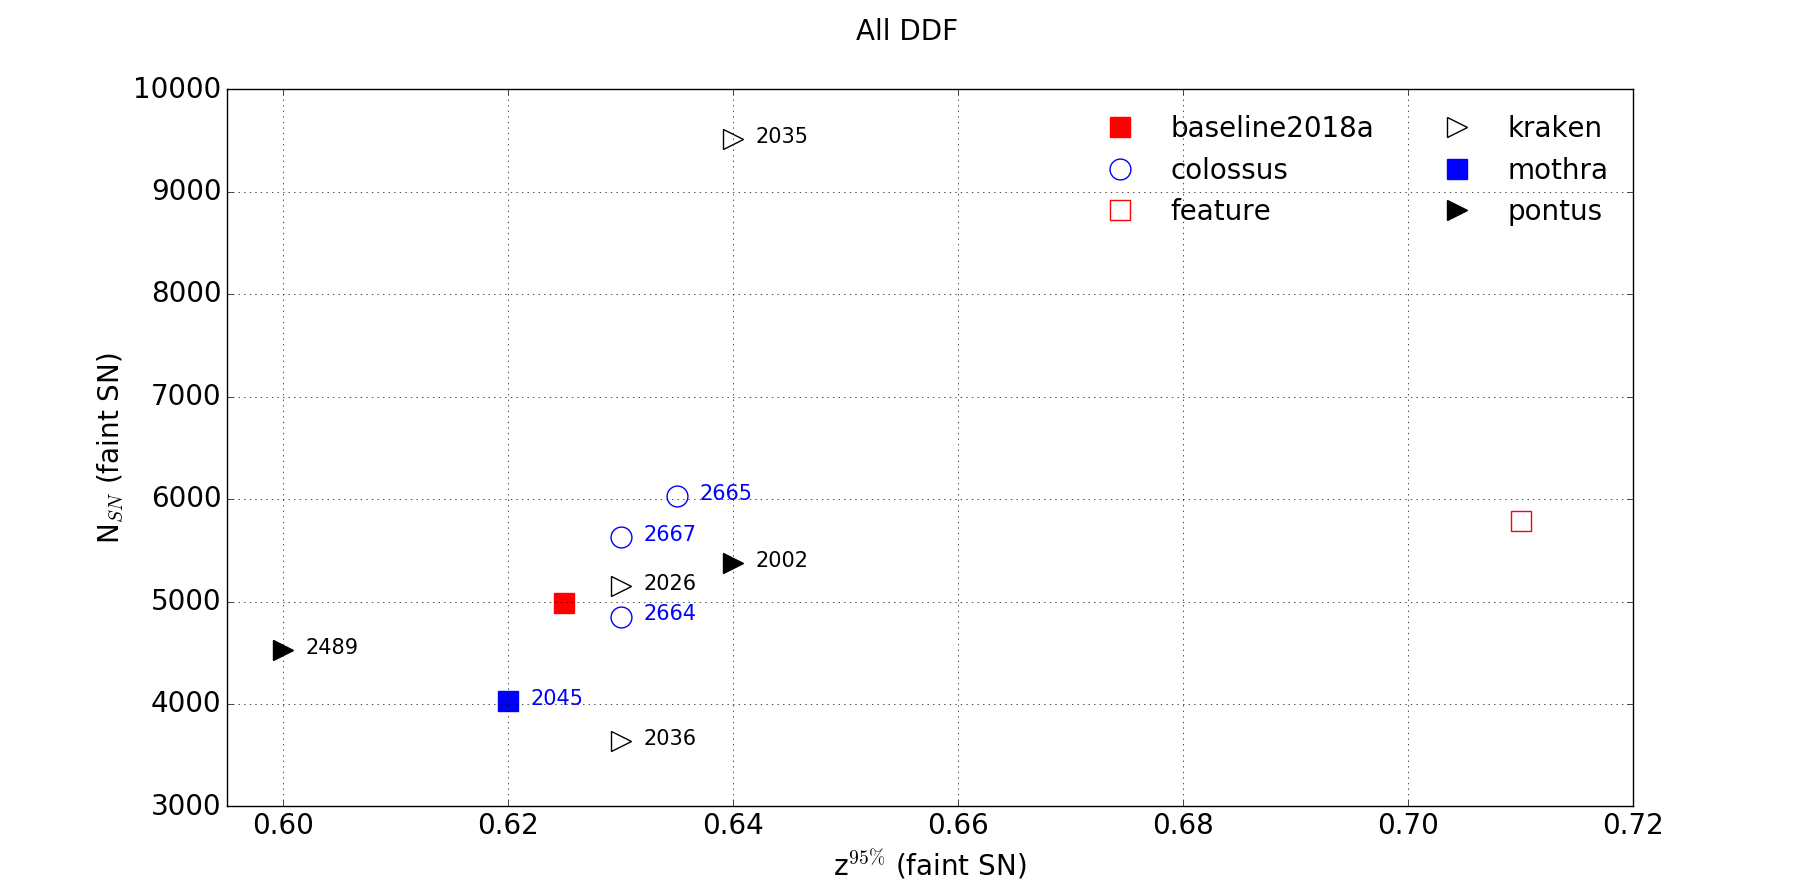
\includegraphics[width=\linewidth]{Z95_NSN.png}
    \caption{Median 95\% redshift limit corresponding to an observation of 95\% of the medium (top) and faint (bottom) supernovae sample as a function of the number of supernovae (top: $z\leq z_{0.95}^{med}$); bottom: $z\leq z_{0.95}^{faint}$)}
    \label{fig:z95}
  \end{center}
\end{figure}

When considering all DDF the best observing strategy (see Table \ref{tab:ddf_nsn}) is as expected kraken\_2035 (30K after ten years) since this simulation considered 9 DDFs whereas all others observed 4 to 5 fields. One may observe that extrapolating a four fields configuration results (like the ones obtained with \feature) to a 9 DDF observing strategy will probably lead to an overestimation of the resulting number of well-measured type Ia supernovae. It is indeed difficult to maintain the same quality (in terms of cadence, season length and thus depth) when moving from a 4 to a 9 DDF strategy.

\begin{table*}[!htbp]
  \caption{Number of well-measured \sne~after ten years. The top 3 observing strategies are listed.}\label{tab:ddf_nsn}
  \begin{center}
  \begin{tabular}{c|cc||cc}
    \hline
    \hline
    Rank & \multicolumn{2}{c}{4 DDF} & \multicolumn{2}{c}{All DDF} \\
    \hline
    
     & Observing strategy & $N_{SN}$ & Observing strategy & $N_{SN}$ \\
     \hline
     1 & colossus\_2667 & 16218 $\pm$ 2698 & kraken\_2035 & 30255 $\pm$ 3453 \\
     2 & \feature & 15723 $\pm$ 2509 & colossus\_2665 & 19033 $\pm$ 2724 \\
     3 & colossus\_2665 & 15149 $\pm$ 2424 & colossus\_2667 & 18214 $\pm$ 2797 \\
    \hline
  \end{tabular}
 
  \end{center}
\end{table*}

Another way to assess the quality of an observing strategy is to estimate the redshift detection limit for faint or medium supernovae. On the Figure \ref{fig:z95} are  displayed the 95\% redshift limit (ie corresponding to the detection of 95\% of the medium and faint supernovae sample) as a function of the number of supernovae (with  $z\leq z_{0.95}$). Huge variations among and inside strategies are observed. This plot reflects the quality of the proposed cadences. It seems that \redshift~of 0.7-0.75 may be reached with four fields. \feature~tend leads to the highest redshift limits and to the most homogeneous results among the fields and seasons. 

\newpage

%% w0-wa FoM
\mybox(w0-wa Figure of Merit,)


In order to assess the impact of the cadence on the cosmological analysis possible with supernovae, we compute the Dark Energy Task force figure of merit in the dark energy parameters $w_0-w_a,$ for a few scenarios.
In the first instance, the supernova sample is simulated following roughly the same prescription as that outlined in the recent Science Requirements Document \cite{descsrd}, with small changes to the host redshift selection. For the SRD we adjusted the survey size simulated to ensure roughly 112 000 SNe after host selection cuts from a 4MOST-like ground based telescope. This is the largest determinant of the final size, and so in order to test for differences in the survey strategy we initially doubled the survey size simulated, and then tested a few cadences without requiring any spectrosopic host redshift. This was to ensure that the host-$z$ follow up was not the most important characteristic.
In addition, we imposed a more restrictive cut on the fitted colour in the SAL2T fit from $\sigma(c) < 0.08$ to $\sigma(c) < 0.05.$ Insodoing we are forcing that the supernovae that survive are of higher quality than in the DESC SRD.
Finally, we include only statistical errors: for speed of computation we have neglected the astrophysical systematics; this will be relaxed in future versions


\begin{figure}[htbp]
  \begin{center}
    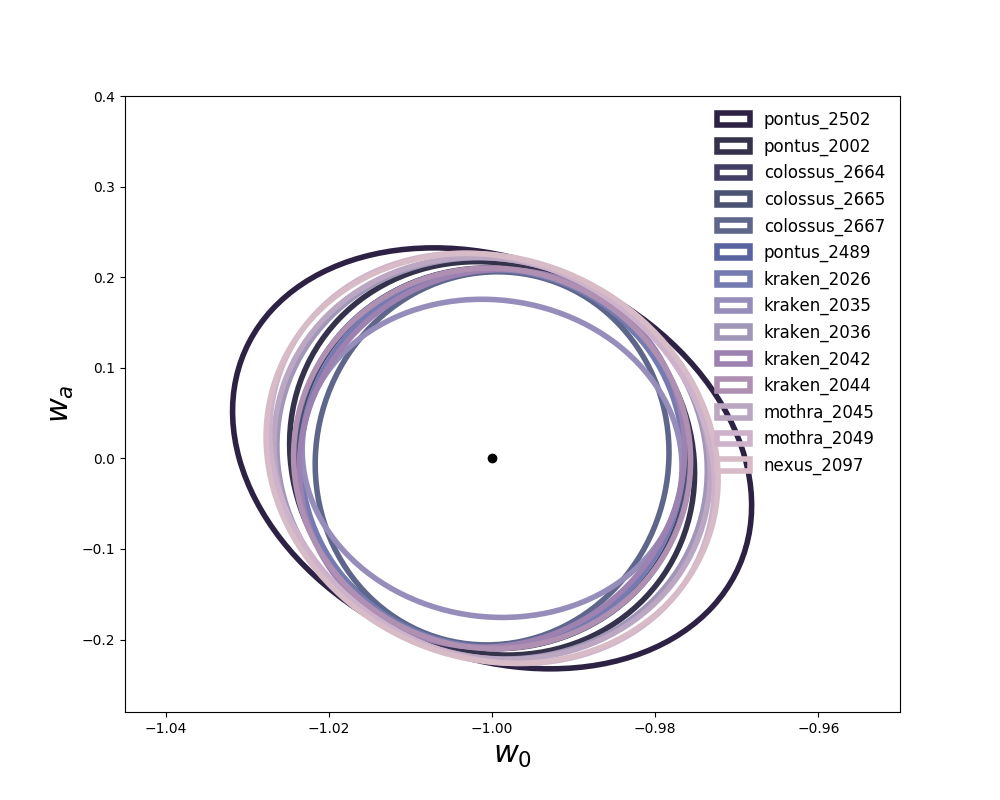
\includegraphics[width=0.7\textwidth]{FM_plot_cadence_updated.png}
    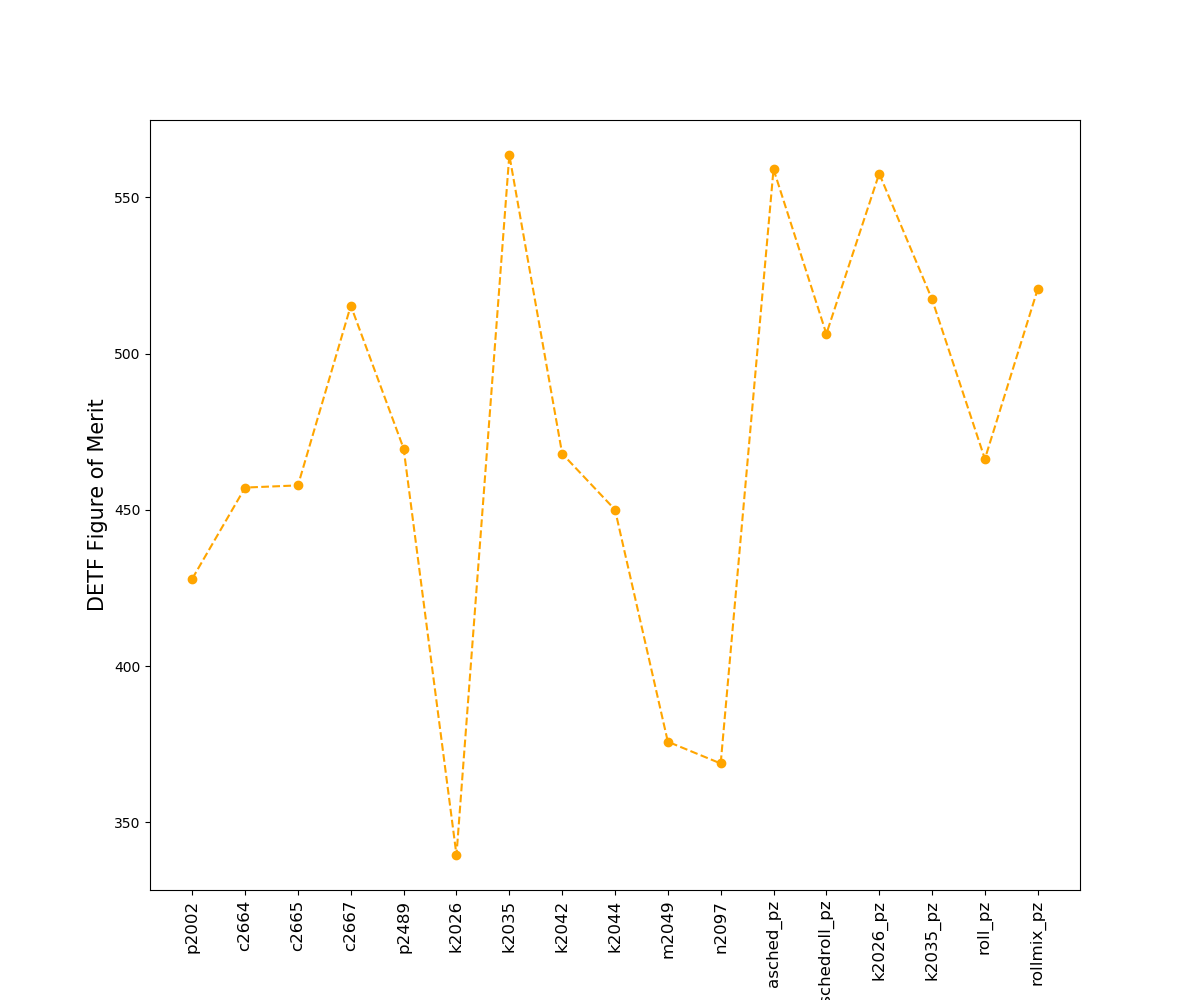
\includegraphics[width=0.7\textwidth]{FoM_cadence_updated.png}
    \caption{Cosmology constraints across cadence types: the ellipses in the $w_0-w_a$ plane (a) and the dark energy figure of merit is shown (b) are shown. \textbf{[RH: plot to be changed once NSERC comes back online 10/18]}}
    \label{fig:w0wa}
  \end{center}
\end{figure}


In the figure above, we see that the largest difference in the Figure of Merit \ref{fig:w0wa} we find is a factor of two between the highest FoM (kraken\_2035) and the lowest FoM (nexus\_2097). The lowest-performing strategy has two alternating bands in declination, switching in alternate years, which is expect to perform poorly. 

In order to test more strongly the impact of the wide field cadence on the overall cosmology, we ran simulations including \textit{only the WFD survey} in addition to a low-$z$ (e.g. Foundation-like) data set. We compared the cosmology results from the WFD+Foundation surveys for the {\tt kraken\_2026, kraken\_2035} and {\tt altsched, altsched\_rolling} cadences. Finally we show the results with and without spectroscopic host redshift selection for the baseline {\tt kraken\_2026} survey. \textbf{[RH: these cosmosis runs will proceed on NSERC on 10/18 after cori comes back up]}

\newpage

%% Photometric classification
\mybox(Photometric Classification,)

The motivation for this work comes from the desire to identify as many \sne in
order to help constrain the nature of Dark Energy.
LSST will observe many more Supernova than ever before, but at a rate that is
not feasible for all of these transients to be spectroscopically followed up and
classified. Thus, the ability to classify these objects photometrically will be very
important. If one can obtain a greater set of \sne, an updated Hubble
digram plot can be produced and the fundamental parameters of the cosmological
model can be tested further.

In order to conduct this analysis, use of
{\tt SNANA}\cite{kessler2009snana}, has been employed to generate the latest light curves that
correspond to different cadences runs from \opsim outputs. The generated light
curves are then used as inputs in {\tt snmachine}, a photometric
classification pipeline \cite{lochner2016photometric}.

By interpolating the sampled light curved with Gaussian processes and then
applying a wavelet decomposition to these interpolated light curves, one obtains features
that could be provided to a classifier, in this case a Random Forest algorithm.
For performance, the dimensions of these features were reduced further with a principle
component analysis and then these reduced features were provided as inputs to the algorithm.
To ensure a controlled test,
for each cadence run, a classifier was trained on 2000 light
curves only and then tested on the remaining set of light curves that were in the
corresponding dataset produced from {\tt SNANA}, in relation to specific
\opsim cadence simulation.
The performance of the interpolation is directly affected by the amount of
samples one has on the light curve. More samples improve the reliability of the Gaussian processes and thus provide better features via the wave
decomposition. Hence short sampling of light curves is important to classify transients. erstood that in order to classify transients, short
sampling of a light curve is important. It is even crucial for early classification leading to possible spectroscopic follow up.


\begin{figure}[htbp]
  \begin{center}
    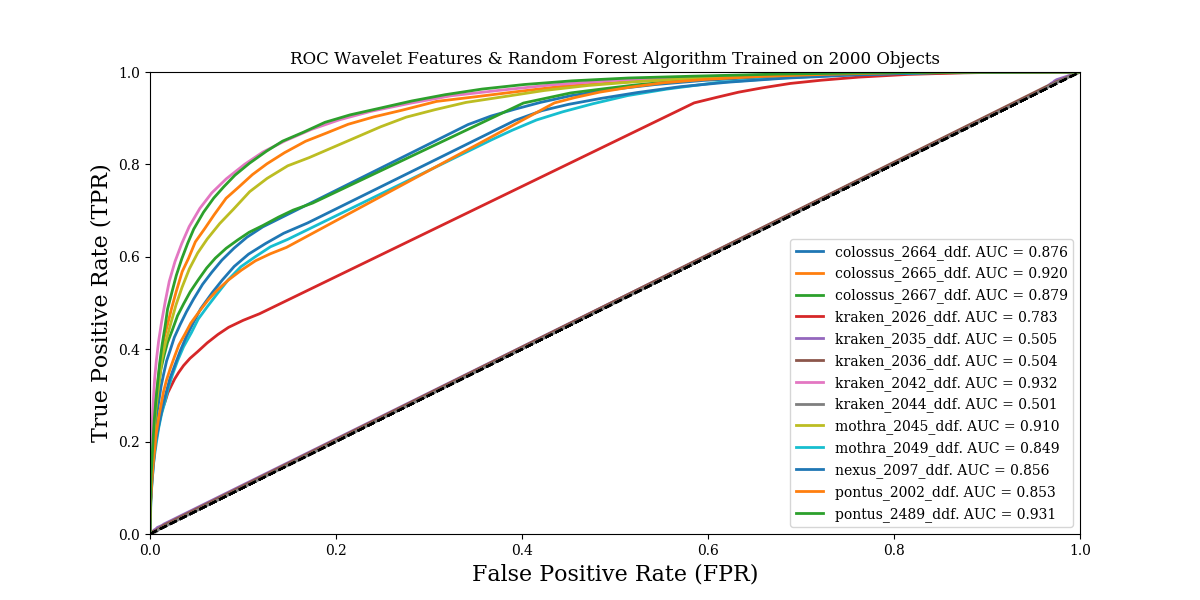
\includegraphics[width=0.9\linewidth]{photometric_classification_roc_results_ddfY1.png}
    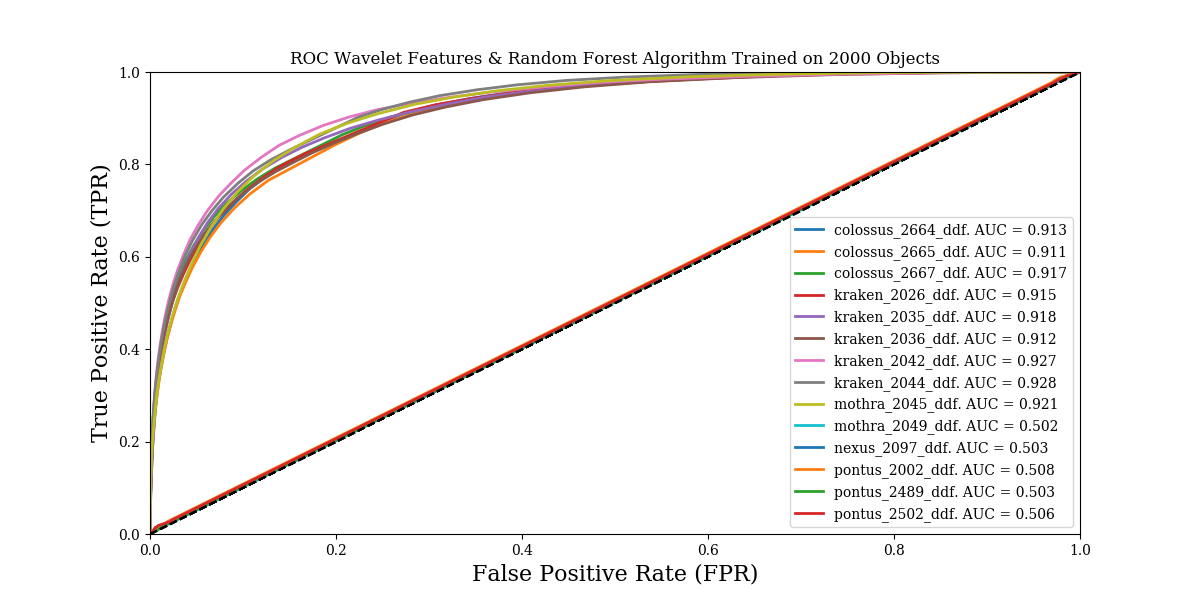
\includegraphics[width=0.9\linewidth]{photometric_classification_roc_results_ddfY10.png}
    \caption{Comparison for the DDFY1 (top) and DDFY10 (bottom) ROC curves}
    \label{fig:rocs}
  \end{center}
\end{figure}


Figure \ref{fig:rocs} (top) ~shows the comparative classification performance between 13 cadences for the Deep
Drilling Fields of Year 1 whereas Figure \ref{fig:rocs} (bottom) ~compares the same
cadences for the Deep Drilling Fields over the entire survey. The area under the Receiver Operating Characteristic (auROC) curves were chosen as the metric
to evaluate the performance. It was felt this single scalar would be most useful
for being able to differentiate the ability of the various cadence strategies
to perform photometric classification.

The results for the DDFY1 case show a significant difference in classification
performance between cadences, with {\tt kraken\_2042} being most favourable.
This cadence has single 30 second snapshots in all bands, thus providing better
sampling along the light curve in all bands. This is one of the elements that could explain
the good performance, and further studies are being carried out to explore which
other elements of cadence result in better classification performance.

If we look at the 10 year survey results, it can be seen there is
little that differentiates the cadences in regard to classification performance.
However, the best performing cadence models are {\tt kraken\_2044} and
{\tt kraken\_2042} which again can be expected from the discussion above.

Further analysis was also done on Wide-Fast-Deep (WFD) cadence runs with work in
progress for models trained on DDF and then tested on WFD.

This research can be taken further in several ways and there are plans to
continue this analysis for new \opsim simulation runs.  In addition, it is
of interest to investigate how the classification performance changes through
time and to compare the results for earch year of the survey. Furthermore,
varying the training set size could have an impact on how well one does for
classification and so this is an area for possible further study.
Finally it would be beneficial to understand how the individual properties of each cadence
strategy affect classification.



\newpage

%% Peculiar velocity (I)

\mybox(Peculiar velocity (I),)

Peculiar velocities provide a measure of $f\sigma_8$, which in turn probes gravity.  As precise distance indicators Type~Ia supernovae (SNe~Ia)
can provide precise peculiar velocities of their host galaxies.

The  expected precision of $f\sigma_8$ using LSST-discovered SNe~Ia is estimated using
the Fisher information matrix of a random Gaussian field with mean zero and covariance $C(k)$ parameterized by $\lambda$ is
\begin{equation}
F_{ij} = \frac{V}{2}\int \frac{d^3k}{(2\pi)^3} \text{Tr}\left[ C^{-1} \frac{\partial C}{\partial \lambda_i} C^{-1}
\frac{\partial C}{\partial \lambda_j} \right].
\end{equation}
The covariance
\begin{equation}
C = P_{vv}(k) + \frac{\sigma^2}{n}
\end{equation}
has contributions from the power spectrum, noise in the velocity measurement, and the density of velocity probes.
In the sample variance limit for a sample with fixed depth, the variance in $f\sigma_8$ (and other $\lambda$ parameters)
is thus inversely proportional to the survey solid-angle $\Omega$, whereas
in the shot-noise limit the variance is inversely proportional to $\Omega n^2 \propto N^2/\Omega$, where $n$ is the number density,
and $N$ is the total number of supernovae.  

We consider a maximum redshift of $z=0.2$ because over ten years the noise is not shot-noise dominated, meaning that the differential improvement
in the precision of
$f\sigma_8$ due to a lower-redshift supernova is greater than that due to a high-redshift supernova.  Following all LSST SNe~Ia below this redshift 
likely saturate available follow-up resources.
Our calculations are thus based on the number and solid-angle of $z<0.2$ supernova pre-maximum discoveries 
for the survey candidates provided by the Project.  Based on these numbers we calculate the Figures of Merit in
both sample and shot-noise limits, normalized to ``baseline2018a''.
After 10 years,
LSST supernovae are at neither extreme; we thus adopt the average of the two FoM's as what we advocate for the survey.
These averages for a select set of surveys are shown in Figure~\ref{fig:fom}.

\begin{table}
\caption{SN~Ia Figures of Merit of Project survey candidates
in  the shot-noise and the survey-variance limits.  The final column is the average
of the two Figures of the Merit.\label{table:ref}}
\centering
\begin{tabular}{|c|rrr|}
\hline
Survey & FoM (shot) & FoM (survey) & FoM (avg)\\
\hline
altsched\_good\_weather & 2.914 & 0.91 & 1.912  \\
alt\_sched\_twi & 2.816 & 0.927 & 1.871  \\
alt\_sched & 2.788 & 0.91 & 1.849  \\
altsched\_18\_\_90\_40 & 2.594 & 1.187 & 1.89  \\
altsched\_18\_\_90\_30 & 2.581 & 1.187 & 1.884  \\
kraken\_2044 & 2.565 & 1.162 & 1.863  \\
colossus\_2667 & 2.365 & 1.004 & 1.684  \\
pontus\_2489 & 2.052 & 0.97 & 1.511  \\
blobs\_mix\_zmask10yrs & 1.432 & 1.008 & 1.22  \\
cadence\_mix\_10yrs & 1.012 & 1.012 & 1.012  \\
rolling\_mix\_10yrs & 0.958 & 1.011 & 0.984  \\
kraken\_2026 & 0.947 & 0.838 & 0.892  \\
rolling\_mix\_75\_10yrs & 0.85 & 1.007 & 0.928  \\
altsched\_rolling\_good\_weather & 0.815 & 0.92 & 0.868  \\
colossus\_2664 & 0.814 & 0.884 & 0.849  \\
tms\_drive\_10yrs & 0.806 & 1.09 & 0.948  \\
alt\_sched\_rolling & 0.804 & 0.92 & 0.862  \\
colossus\_2665 & 0.797 & 0.861 & 0.829  \\
kraken\_2042 & 0.794 & 0.858 & 0.826  \\
baseline2018a & 0.779 & 0.834 & 0.807  \\
kraken\_2035 & 0.705 & 0.823 & 0.764  \\
mothra\_2049 & 0.671 & 1.161 & 0.916  \\
tight\_mask\_10yrs & 0.646 & 1.155 & 0.901  \\
tight\_mask\_simple\_10yrs & 0.6 & 1.141 & 0.871  \\
rolling\_10yrs & 0.581 & 0.838 & 0.709  \\
%kraken\_2036 & 0.437 & 1.141 & 0.789  \\
tms\_roll\_10yrs & 0.424 & 1.119 & 0.771  \\
nexus\_2097 & 0.28 & 1.166 & 0.723  \\
%mothra\_2045 & 0.226 & 1.134 & 0.68  \\
pontus\_2002 & 0.224 & 1.157 & 0.691  \\
feature\_rolling\_twoThird\_10yrs & 0.187 & 1.104 & 0.645  \\
feature\_rolling\_half\_mask\_10yrs & 0.175 & 0.987 & 0.581  \\
%pontus\_2502 & 0.132 & 1.107 & 0.62  \\
minion\_1016 & 0.093 & 1.109 & 0.601  \\
blobs\_same\_10yrs & 0.064 & 0.859 & 0.462  \\
blobs\_same\_zmask10yrs & 0.048 & 0.859 & 0.453  \\
feature\_baseline\_10yrs & 0.025 & 0.642 & 0.334  \\
\hline
\end{tabular}
\end{table}

\begin{figure}[htbp]
   \begin{center}
   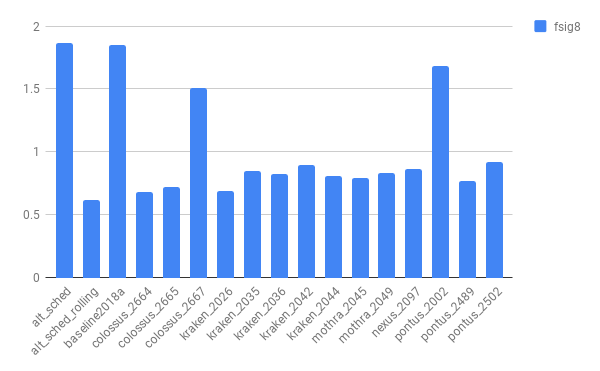
\includegraphics[scale=0.5]{chart.png} % requires the graphicx package
   \caption{Figure of Merits of Select Surveys}
   \label{fig:fom}
   \end{center}
\end{figure}

We are in the course of refining the Figure or Merit, taking into account survey geometry, combining both survey variance and shot noise.
Any significant changes in our findings will lead to an update of our relative ranking of the surveys.

\newpage
%% Peculiar velocity (II)
\mybox(Peculiar velocity (II),)


Upcoming wide field surveys will find a large number of supernovae, and will have the ability to trace large scale structure. The best methods to do so need to be explored. In particular, the interesting methods will probably use both the distance  scales measured by supernovae using their standard candle properties and their properties as tracers of large scale structure simultaneously for the same supernova. One such probe is a probe of peculiar velocity correlations using SNIa, where the standard candle property is used to derive the distance scale, while the measured redshift (spectroscopic or photometric) is used simultaneously to gauge the peculiar velocity of the SNIa (which is potentially the peculiar velocity of the host galaxy). The spatial correlation of such peculiar velocities is related to the matter over-density at the location through the Poisson Equations, and thus can be used to constrain the over-densities and the growth function. This can be used to constrain the cosmology (for example, see \cite{2011PhRvD..83d3004B}).

In what follows, we heavily rely on \cite{2011PhRvD..83d3004B} to estimate the uncertainties in the estimate of pairwise velocities as a function of the comoving separation in bins of redshift. The expected signal is largest at low redshift, where the signal of the peculiar velocity is large compared to the recession velocity of the Hubble flow.  The uncertainty on the estimated pair-wise radial velocities of tracers separated by a comoving distance $r$ Mpc is given by
\begin{equation}
v_{\rm{est}} \approx 2 \times \sigma_{v_{\rm{los}}} / N^{1/2}(r, z_{\rm{cosmo}})
\end{equation}
where $N(r,z_{cosmo})$ is the number of pairs of SNIa separated by a comoving distance of $r~\rm{Mpc}$
at a cosmological redshift of $z_{\rm{cosmo}},$ and $\sigma_{v_{\rm{los}}}$ is the uncertanty in the
measurement of the line of sight velocity of SNIa. Thus, estimating the signal-to-noise ratio depends on the size of both $N(r, z_{cosmo})$ and $\sigma_{v_{\rm{los}}}$. We have estimated these quantities for different cadences. 

To calculate the number of pairs of detected SNIa at a given comoving separation in redshift bins we need a realization of SNIa positions and velocities in the universe that are consistent with the underlying correlations in large scale structure. To obtain these correlations, we start from an extra-galactic catalog based on large-scale structure simulations. We add SNIa in the galaxies of the simulated extra-galactic catalog using a prescription based on some observed relationships of the SNIa - host galaxy connection. The SNIa-host galaxy connection is an area of active research from large SNIa surveys; consequently all the host galaxy properties observed are not found in the extra-galactic catalogs we can use. Consequently, we start with a simple realization prescription based on known aspects of the connection and easily observed properties of SNIa. This preserves two gross properties of SNIa distributions: the volumetric abundance rate as a function of redshift and the fact that SNIa are more abundant in galaxies with larger stellar mass. As a result of this work, we obtain a catalog of SNIa over a sky area of $A_{cat}.$

We parametrize the system by a median efficiency of detection $\epsilon = N_{det}/N_{sim}$ from other comprehensive simulations being used for supernova cadence studies, which are in turn related to a footprint area $A_{survey}$ covered by the particular observing strategy. For our purposes, we choose the footprint area of the sky where the observing strategy has at least $500$ visits over ten years.\footnote{This is the region over which the SNANA simulations run.}
Therefore, we work out how the number of detected pairs scale with $A_{survey}$ and $\epsilon$ and use this information to correct the theoretical values in $N_{pairs}$ counted in the extra-galactic catalog SN. The number of pairs of SNIa separated by a distance $r$ Mpc can be found by iterating through the SNIa ($\sim N_{SN}$), and finding the number of SNIa lying in a shell of radius $r$ Mpc with a thickness $dr$ Mpc around it, and dividing by two to avoid double counting. Using the number density of detected SN $n^{det}_{SN} \equiv N_{det}/Vol = \epsilon N_{SN}/Vol = \epsilon n_{SN},$ where $n_{SN}$ is the number density of the SNIa independent of survey parameters the number of pairs of detected SNIa with separation $r$ Mpc is:
%\begin{equation}
    $$
    N_{pairs} \propto N_{det} \times {n_{det}} \propto A_{survey} \epsilon^2 {n_{SN}}.
    $$
%\end{equation}
Thus, the estimate for number of pairs is given by
%\begin{equation}
$$
    \hat{N}_{pairs} = \left( A_{survey} / A_{catalog} \right)\hat{\epsilon}^2 \times N_{pairs}^{catalog}
    $$
%\end{equation}
where the estimate $\hat{\epsilon}$ comes from the ratio $N_{det}/ N_{simulated}$ in SNANA. 

We now consider the light curve quality with and without ground-based follow up.
If we were to get perfect light curves with lots of well observed points, as might be obtained if all low-$z$ SNIa are followed up photometrically with a different telescoper, then the appropriate metric is 
\begin{equation}
    m_{follow} \propto A_{survey} \times \epsilon^2,
\end{equation}
while if LSST is the only photometric instrument, the appropriate metric (calculated in Table \ref{tab:cadence_metrics}) is
\begin{equation}
    m_{LSST} \propto A_{survey} \epsilon^2 /(1.0 + \left(\sigma_{lc}/0.1\right)^2)^{1/2}
\end{equation}



\begin{table}
\begin{center}
\begin{tabular}{|c|c|c|}
    \hline
     cadence &  Metric (photo follow-up) &  metric (LSST Only) \\
     \hline
    %mothra\_2045 & 2.465604 & 1.495344  \\
	%kraken\_2036 & 2.696759 & 1.637113  \\
	nexus\_2097 & 3.047014 & 1.832897  \\
	mothra\_2049 & 3.119186 & 1.890817  \\
	%pontus\_2502 & 3.14715 & 1.910531  \\
	colossus\_2665 & 3.558642 & 2.192984  \\
	kraken\_2026 & 3.603123 & 2.231208  \\
	colossus\_2664 & 3.617946 & 2.229529  \\	
	kraken\_2035 & 3.638301 & 2.242073  \\
	kraken\_2042 & 3.714791 & 2.305959  \\
	pontus\_2002 & 3.721372 & 2.248261  \\
	pontus\_2489 & 4.131681 & 2.602565  \\
	colossus\_2667 & 4.228459 & 2.677912  \\
	kraken\_2044 & 4.355133 & 2.700822  \\
     \hline
\end{tabular}
\end{center}
\caption{Peculiar velocity metrics for various cadences: Here `photo follow-up` implies that light curves of d
etected supernovae are perfect due to photometric follow-up with a different telescope. The right hand column 
gives the metric `(LSST Only)', where only LSST observations are assumed; the uncertainty on the distance modu
lus comes from the median uncertainty from LSST-only fits.}
\label{tab:cadence_metrics}
\end{table}


\vspace*{10cm}
\newpage

%% Overlap with 4MOST

\mybox(Overlap with 4MOST extragalactic surveys,)

The 4MOST facility will be a highly multiplexed, optical, fibre-fed
spectrograph mounted on the 4-metre VISTA telescope. It is due to
start operations at the end of 2022. Its wide field of view (4.1 sq
deg), high multiplex (1600 fibres feeding low-resolution spectrographs
suitable for extragalactic science plus $\sim 800$ fibres feeding a
high-resolution spectrograph, primarily for galactic science) and
geographical location (near the Paranal site in Chile) makes 4MOST an
ideal spectroscopic follow-up facility for LSST. The scientific
synergy potentially covers a very wide variety of science goals. Here
we focus on the synergy for follow-up of transients and varying
sources.

The 4MOST-TiDES survey plans to piggy-back on other 4MOST
extragalactic surveys, and will use a small subset of the fibres in
each pointing to observe live transients and the host galaxies of
previously-discovered transients. The 4MOST extragalactic surveys will
be carried out over a large fraction of the southern sky, shown in
Figure~\ref{fig:4most_sky}.  There is also a component of TiDES that aims
to obtain spectral time-sequences of AGN in 4MOST's deep fields (that
are likely to coincide with at least a subset of LSST's deep fields,
TBD), for reverberation mapping.

\begin{figure}[!htbp]
\begin{center}
  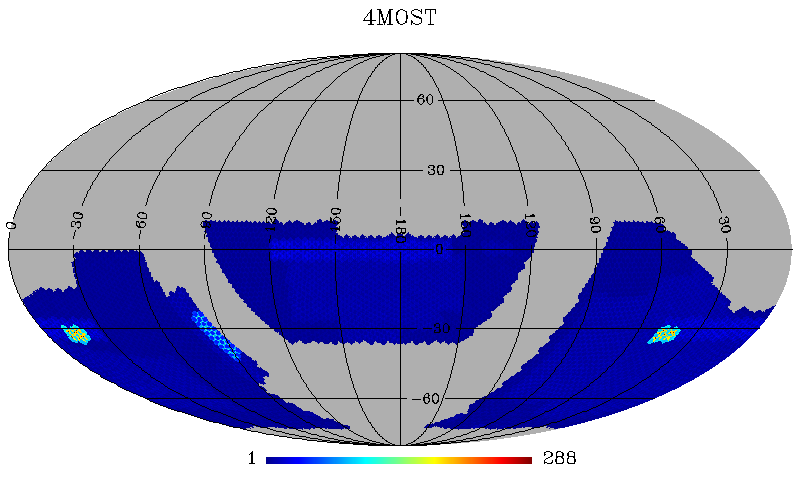
\includegraphics[width=10.0cm]{4most_fndep.png}
\end{center}
\caption{One realisation of the sky coverage of 4MOST extragalactic
  surveys, colour coded by number of visits. This is based on
  4MOST-4FS survey simulation round9/c/run01 dated 2018-5-14. Note
  that the 4MOST survey design is still in progress and the map is
  likely to change.}
\label{fig:4most_sky}
\end{figure}

There is a preference for 4MOST to observe within the approximate
declination range seen in Figure~\ref{fig:4most_sky} for several
reasons. One is not to duplicate other facilities in the North (such
as DESI, Subaru-PFS and WEAVE). Another is that the winds from the
north at Paranal can make it difficult to observe in that
direction. Similarly, 4MOST prefers not to observe far South because
of inefficiency when observing at high airmass. The 4MOST Atmospheric
Dispersion Compensator works optimally upto zenith distances of 55
degrees, equivalent to airmass of $\sim1.75$. At larger airmasses,
light is lost at the ends of the spectrum. Because VISTA is at
latitude $\sim -24.7$ degrees, one can therefore observe theoretically
to declination of $\sim -80$ degrees at the meridian. In practice
4MOST will not go much below declination of $-70$ degrees, except in
the Magellanic Clouds, as observations get much harder to schedule if
one wants to stay beyond airmass $\sim 1.75$ for an hour. However,
there could be exceptions if, for example, there was an interesting
deep field a bit north or south of the current range.

\begin{comment}
In addition to the extragalactic surveys, 4MOST will survey the Milky
Way disk area with the same 1600 fibres feeding low-resoution + 800
fibres feeding high resolution spectrographs, but this will be mainly
in bright time and geared toward brighter targets and hence less
suitable for extra-galactic follow-up. However, this survey might be
interesting for follow-up of stellar variables.

Finally, we note that a Call for Letters of Intent for 4MOST community
observations is expected to be opened next summer (2019).
\end{comment}

For the LSST (WFD) surveys we used each OpSim simulation (with a dither
pattern superimposed that gives a high spatial uniformity of depth) to
make a healpix map\footnote{NSIDE=256 (approx. 0.052 sq deg resolution)}, and kept all healpixels with more than 500 visits
over 10 years. For 4MOST, we used the most recent 4MOST 4FS simulation,
(round9/c/run01 dated 2018-5-14) and made a Healpix map using the
central coordinates of each 4MOST tile, and assuming a hexagonal field
of view with area 4.1 sq deg. Each Healpixel with one or more visits
was kept.
 

We then calculated number of overlapping healpixels and multiplied by the
spatial area of one healpixel to give the overlapping areas shown in
Table~\ref{tab:4most_overlap}.



\begin{table}[!htbp]
  \begin{center}
 \caption{Overlapping areas between LSST WFD and 4MOST extragalactic surveys}\label{tab:4most_overlap}
\begin{tabular}{cc}\hline \hline
  LSST OpSim run & Overlapping area (sq deg) \cr\hline \hline
  %mothra\_2045   &	11702 \cr
  colossus\_2667 &	12644 \cr
kraken\_2026   &	12644 \cr
%kraken\_2036   &        12644 \cr
pontus\_2489   &	12644 \cr  
%pontus\_2502   &	12644 \cr
colossus\_2664 &        12805 \cr
colossus\_2665 &	13096 \cr
pontus\_2002   &	15000 \cr
  \hline
\end{tabular}
\end{center}
\end{table}



4MOST will typically visit each part of the sky twice, for about one
hour exposure ($3\times$ 20 mins) exposures each time (but we
emphasise again that the details of the 4MOST survey are still under
discussion). Clearly, for follow-up of live transients it is important
that 4MOST observes in the areas of sky the LSST has visited recently
(within the lifetime of the transients concerned). For example if LSST
follows a rolling cadence then to maximise trabnsient science, 4MOST
should observe in the same declination range.  Coordination of LSST
and 4MOST surveys is essential.
 	 
 	 
Of the LSST cadence simulations considered, Pontus\_2002 gives the
largest overall spatial overlap, of approx. 15,000 sq deg, compared to
approximately 12,000-13,000 sq deg for the other surveys. The extended
declination range of Pontus\_2002 increases the overlap with 4MOST,
but goes a little too far in that some of extended LSST area is then
not covered by 4MOST.

As stressed above, temporal coordination of the 4MOST and LSST surveys is
essential if transient science is to be maximised.

\newpage

\bibliographystyle{plain}
\bibliography{biblio}



\end{document}
